%%%%%%%%%%%%%%%%%%%%%%%%%%%%%%%%%%%%%%%%%
% Vertical Line Title Page 
% LaTeX Template
% Version 1.0 (27/12/12)
%
% This template has been downloaded from:
% http://www.LaTeXTemplates.com
%
% Original author:
% Peter Wilson (herries.press@earthlink.net)
%
% License:
% CC BY-NC-SA 3.0 (http://creativecommons.org/licenses/by-nc-sa/3.0/)
% 
% Instructions for using this template:
% This title page compiles as is. If you wish to include this title page in 
% another document, you will need to copy everything before 
% \begin{document} into the preamble of your document. The title page is
% then included using \titleGM within your document.
%
%%%%%%%%%%%%%%%%%%%%%%%%%%%%%%%%%%%%%%%%%

%----------------------------------------------------------------------------------------
%	PACKAGES AND OTHER DOCUMENT CONFIGURATIONS
%----------------------------------------------------------------------------------------

\documentclass{report}

\usepackage{cite,graphicx}
\usepackage[chapter]{algorithm}
\usepackage{url,float}
\usepackage{hyperref}
\usepackage{uithesis}
\usepackage{listings}
\usepackage[nodayofweek,level]{datetime}
\usepackage[bahasai]{babel}
\selectlanguage{bahasai}
\renewcommand{\bibname}{Daftar Referensi}
\renewcommand{\contentsname}{Daftar Isi}
\renewcommand{\listfigurename}{Daftar Gambar}
\renewcommand{\listtablename}{Daftar Tabel}
\renewcommand\lstlistingname{Program}
\renewcommand\lstlistlistingname{Daftar Program}
%\def\lstlistingautorefname{Program.}
\renewcommand{\chaptername}{BAB}
\renewcommand{\figurename}{\bo{Gambar}}
\renewcommand{\tablename}{\bo{Tabel}}
\Var{\kataPengantar}{Kata Pengantar}
%
% Hyphenation untuk Indonesia 
%
% @author  Andreas Febrian
% @version 1.00
% 
% Tambahkan cara pemenggalan kata-kata yang salah dipenggal secara otomatis 
% oleh LaTeX. Jika kata tersebut dapat dipenggal dengan benar, maka tidak 
% perlu ditambahkan dalam berkas ini. Tanda pemenggalan kata menggunakan 
% tanda '-'; contoh:
% menarik
%   --> pemenggalan: me-na-rik
%

\hyphenation{
    % alphabhet A
    a-na-li-sa a-tur 
    a-pli-ka-si 
    % alphabhet B
    ba-ngun-an 
    be-be-ra-pa 
    ber-ge-rak
    ber-ke-lan-jut-an 
    ber-pe-nga-ruh 
    ber-o-pe-ra-si
    % alphabhet C
    ca-ri cri-ti-cal
    % alphabhet D
    di-sim-pan di-pim-pin de-ngan da-e-rah di-ba-ngun da-pat di-nya-ta-kan 
    di-sim-bol-kan di-pi-lih di-li-hat de-fi-ni-si
    di-mo-del-kan di-te-rap-kan
    di-ha-rap-kan
    di-e-va-lu-a-si
    di-su-sun
    di-sa-ji-kan
    % alphabhet E
    e-ner-gi eks-klu-sif
    % alphabhet F
    fa-si-li-tas
    % alphabhet G
    ga-bung-an ge-rak
    % alphabhet H
    ha-lang-an
    % alphabhet I
    % alphabhet J
    % alphabhet K
    ke-hi-lang-an
    ku-ning 
    kua-li-tas ka-me-ra ke-mung-kin-an ke-se-pa-ham-an
    % alphabhet L
    ling-kung-an
    % alphabhet M
    me-ne-ngah
    meng-a-tas-i me-mung-kin-kan me-nge-na-i me-ngi-rim-kan 
    meng-u-bah meng-a-dap-ta-si me-nya-ta-kan mo-di-fi-ka-si
    meng-a-tur
    meng-a-la-mi
    me-re-pre-sen-ta-si-kan
    men-da-pat-kan
    me-nun-juk-kan
    % alphabhet N
    nya-ta non-eks-klu-sif nu-klir
    % alphabhet O
    o-pe-ra-si
    % alphabhet P
	pe-nye-rap-an 
	pe-ngon-trol
    pe-mo-del-an
    pe-ran  pe-ran-an-nya
    pem-ba-ngun-an pre-si-den pe-me-rin-tah prio-ri-tas peng-am-bil-an 
    peng-ga-bung-an pe-nga-was-an pe-ngem-bang-an 
    pe-nga-ruh pa-ra-lel-is-me per-hi-tung-an per-ma-sa-lah-an 
    pen-ca-ri-an peng-struk-tur-an
    per-siap-an pa-ra-me-ter
    pa-sang-an
    % alphabhet Q
    % alphabhet R
    ran-cang-an
    % alphabhet S
    si-mu-la-si sa-ngat
    % alphabhet T
    te-ngah
    ter-da-pat
    % alphabhet U
    % alphabhet V
    % alphabhet W
    % alphabhet X
    % alphabhet Y
    % alphabhet Z
    % special
}


%----------------------------------------------------------------------------------------
%	TITLE PAGE
%----------------------------------------------------------------------------------------

\newcommand*{\titleGM}{\begingroup % Create the command for including the title page in the document
\hbox{ % Horizontal box
\hspace*{0.2\textwidth} % Whitespace to the left of the title page
\rule{1pt}{\textheight} % Vertical line
\hspace*{0.05\textwidth} % Whitespace between the vertical line and title page text
\parbox[b]{0.75\textwidth}{ % Paragraph box which restricts text to less than the width of the page

{\noindent\Huge\bfseries Pemrograman Python untuk Pengolahan Citra Digital }\\[2\baselineskip] % Title
{\large \textit{Diktat kuliah}}\\[4\baselineskip] % Tagline or further description
{\large \textsc{Dr. Arya Adhyaksa Waskita}} % Author name

\vspace{0.5\textheight} % Whitespace between the title block and the publisher
\begin{figure}[H]

\includegraphics[scale=.2]{pics/logo.png}
\end{figure}
STMIK Eresha - 2020
%Powered by \LaTex

%{\noindent The Publisher \plogo}\\[\baselineskip] % Publisher and logo
}}
\endgroup}

%----------------------------------------------------------------------------------------
%	BLANK DOCUMENT
%----------------------------------------------------------------------------------------

\begin{document}

%\addChapter{\kataPengantar}


\pagestyle{empty} % Removes page numbers

\titleGM % This command includes the title page
\pagenumbering{roman}
\setcounter{page}{0}
\tableofcontents
\listoffigures
\addChapter{Daftar Program}
\lstlistoflistings
\addChapter{\kataPengantar}
%-----------------------------------------------------------------------------%
\chapter*{Kata Pengantar}
%-----------------------------------------------------------------------------%
Diktat kuliah ini hanya merupakan pelengkap agar mahasiswa dapat lebih mudah memahami materi pengolahan citra digital. Penggunaan ilustrasi lain dari perangkat lunak berbayar dapat saja diberikan. Tetapi, karena pertimbangan kemandirian dan lisensi, maka saya memutuskan untuk menyusun diktat ini berbasis pada pustaka berlisensi publik dan berbasis bahasa pemrograman Python, \texttt{scikit-image}. Python dipertimbangkan karena banyak pustaka ilmiah yang sudah umum digunakan dan terus dikembangkan yang berbasis pada Python. Dalam pengolahan citra, selain \texttt{scikit-image}, ada juga \texttt{OpenCV} untuk \textit{Computer Vision}. Dalam pembelajaran mesin, \texttt{scikit-learn} adalah pustaka yang juga banyak digunakan. Bahkan \texttt{tensorflow}, pustaka yang banyak digunakan dalam penelitian \textit{deep learning} juga berbasis pada Python. Saya yakin, dengan mempelajari diktat ini, mahasiswa mampu mandiri dalam penguasaan bahasa pemrograman Python yang pada akhirnya mampu membuat mahasiwa lebih adaptif terhadap pustaka berbasis python, baik untuk tujuan ilmiah maupun bisnis. Mahasiswapun diharapkan menjadi lebih kreatif dalam melakukan penelitian hingga mengembangkan produk perangkat lunak, maupun prototipe perangkat keras cerdas berbasis Python tanpa harus terbebani masalah lisensi.

Secara umum, diktat ini dibagi ke dalam bagian pendahuluan yang membahas tentang sejarah singkat Python yang dilanjutkan ke bagian instalasi. Instalasi ini, meskipun sangat sederhana, terutama pada sistem operasi Linux, dapat menjadi sangat merepotkan bagi beberapa mahasiswa, terutama ketika mereka menggunakan sistem operasi Windows. Karena itu, instalasi akan dilakukan di sistem operasi Windows. Bagian selanjutnya adalah dasar-dasar pemrograman Python, terutama struktur data (\texttt{list}, \texttt{tuple} dan \texttt{dictionary}), interaksi dengan \textit{file}, hingga mempelajari penggunaan fungsi yang terdapat dalam pustaka tertentu. Sedangkan bagian terkahir dari diktat ini akan sepenuhnya diisi dengan fitur pustaka \texttt{scikit-image}, yang saat diktat ini disusun berada pada rilis \texttt{0.17.2}.
\clearpage
Diktat ini tidak ditujukan untuk menjadi rujukan dalam teknik pengolahan citra. Sehingga penjelasan teoritis terkait pengolahan citra akan diberikan dalam porsi yang sangat minim dan hanya ditujukan sebegai pelengkap saja. Selain itu, dalam diktat ini banyak menggunakan sumber dari situs web dan akan disampaikan secara detil alamat sumber tersebut dalam diktat. Diharapkan, mahasiswa tidak takut mencoba karena ada begitu banyak sumber yang dapat digunakan untuk belajar. Hanya kesungguhan kitalah yang akan menjadi pembeda. Akhirnya, selamat mencoba pengalaman baru. 

\vspace*{2cm}
\begin{flushright}
\selectlanguage{bahasai}
Serpong, \today\\[0.1cm]
\vspace*{1cm}
Dr. Arya Adhyaksa Waskita

\end{flushright}


\pagenumbering{arabic}
\chapter{Sejarah Pemrograman Python}

\chapter{Instalasi Python}
\section{Sejarah singkat}
Python dibangun oleh Guido van Rossum (\figurename~\ref{fig:guido}\footnote{\url{https://gvanrossum.github.io/images/guido-headshot-2019.jpg}}) pada sekitar tahun 1980 di \textit{Centrum Wiskunde \& Informatica} (CWI) di Belanda\cite{python3intro}. Nama Python diambil dari program TV favorit Guido yang berjudul '''Monty Pythons Flying Circus''' yang tayang pada kisaran tahun 1969-1974.

\begin{figure}
  \begin{center}
    \includegraphics[scale=.5]{pics/guido-headshot-2019.jpg}
    \caption{Guido van Rossum}
    \label{fig:guido}
  \end{center}
\end{figure}

\section{Interpreter Python}
\label{sec:interpreter}
Seperti telah dijelaskan di bagian Pengantar, instalasi \textit{interpreter} Python dilakukan di sistem operasi Windows 7. Tahapan instalasi ini mengasumsikan bahwa tidak ada kendala apapun terkait sistem operasi. Selanjutnya mahasiwa diminta untuk mengunduh \textit{interpreter} Python melalui laman \url{https://www.python.org/downloads/} sesuai kebutuhannya. 

Mengeksekusi unduhan tersebut akan memunculkan dialog seperti pada \figurename~\ref{fig:install1}. Pastikan untuk memilih konfigurasi \texttt{PATH} secara otomatis agar ketika proses instalasi selesai, \textit{interpreter} Python dapat dijalankan dari mana saja di sistem komputer masing-masing. Untuk kondisi di mana terjadi kesalahan, akan muncul dialog yang memberi kita kesempatan untuk melihat \textit{log}. Buka log tersebut dan lihat sumber dari kesalahan instalasi yang sedang terjadi.

\begin{figure}[h!]
   \begin{center}
     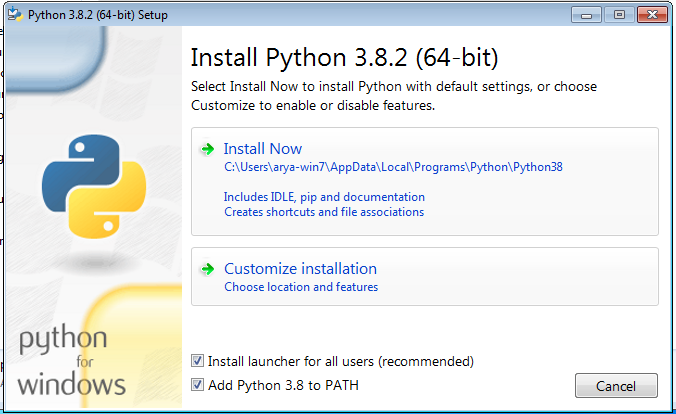
\includegraphics[scale=.5]{pics/installPython1.png}
     \caption{Dialog instalasi \textit{interpreter} Python}
     \label{fig:install1}
   \end{center}
 \end{figure} 

Pilihan opsi \textit{Customize installation} akan menampilkan dialog seperti \figurename~\ref{fig:feature}. Pastikan semua pilihan dipilih. Kemudian, selama proses instalasi berlangsung, pengguna akan disuguhkan dialog seperti \figurename~\ref{fig:installProgres}. Tunggu sampai dialog tanda selesai dikeluarkan seperti pada \figurename~\ref{fig:finish}.

\begin{figure}[h!]
  \begin{center}
    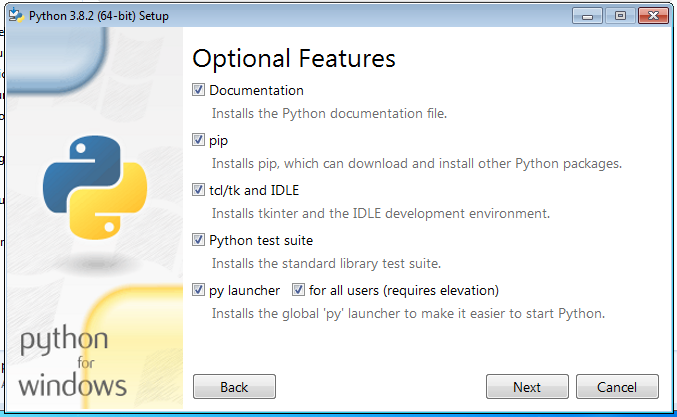
\includegraphics[scale=.5]{pics/featureInstall.png}
    \caption{Pilihan paket pendukung sebelum instalasi dilakukan}
    \label{fig:feature}
  \end{center}
\end{figure}

\begin{figure}[h!]
  \begin{center}
    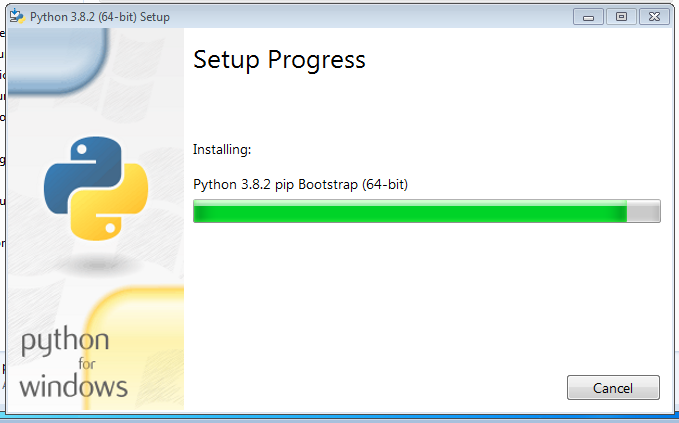
\includegraphics[scale=.5]{pics/installProgress.png}
    \caption{Dialos selama proses instalasi berlangsung}
    \label{fig:installProgres}
  \end{center}
\end{figure}

\begin{figure}[h!]
  \begin{center}
    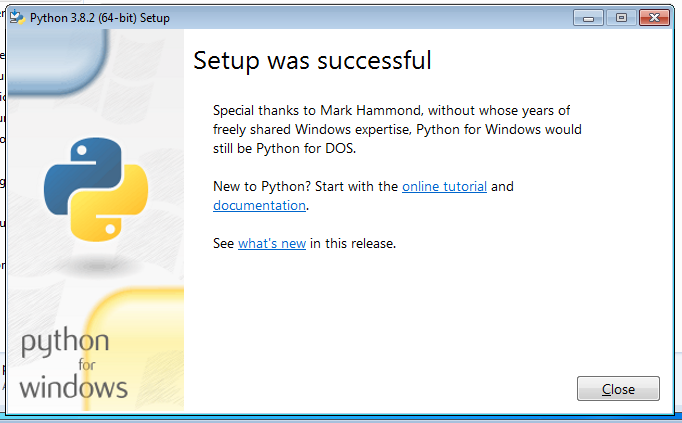
\includegraphics[scale=.5]{pics/installFinished.png}
    \caption{Dialog tanda selesai instalasi}
    \label{fig:finish}
  \end{center}
\end{figure}

Seperti telah ditunjukkan pada \figurename~\ref{fig:install1} tentang informasi lokasi \textit{interpreter} Python diletakkan, dapat juga dibuktikan melalui aplikasi \texttt{CMD} seperti \figurename~\ref{fig:lokasi}. Sedangkan \textit{interpreter} Python dapat diujicobakan dengan menuliskan perintah \texttt{python} di aplikasi \texttt{CMD}. Akan muncul dialog seperti \figurename~\ref{fig:siap}. \textit{Interpreter} Python siap digunakan, ditandai dengan munculnya karakter \texttt{>>>}.

\begin{figure}[h!]
  \begin{center}
    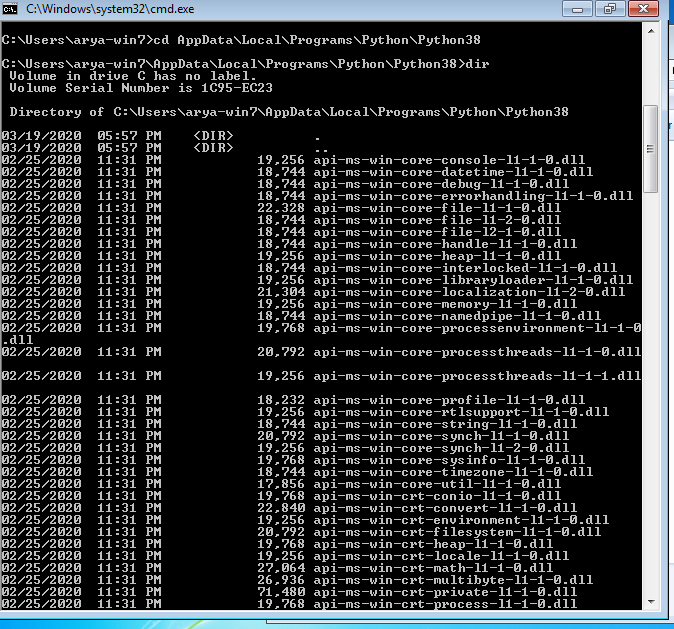
\includegraphics[scale=.5]{pics/installedLocation.png}
    \caption{Lokasi instalasi \textit{interpreter} Python}
    \label{fig:lokasi}
  \end{center}
\end{figure}

\begin{figure}[h!]
  \begin{center}
    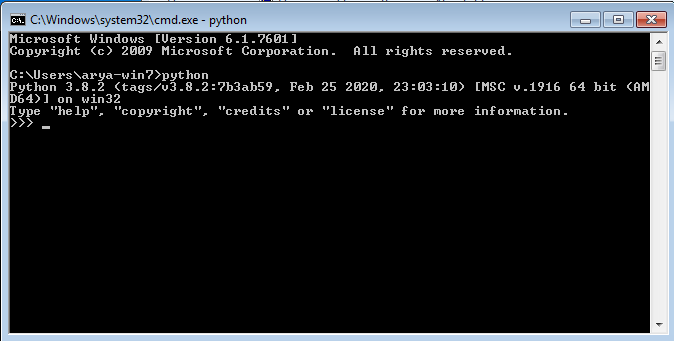
\includegraphics[scale=.5]{pics/pythonAktif.png}
    \caption{\textit{Interpreter} Python siap digunakan}
    \label{fig:siap}
  \end{center}
\end{figure}

Tahapan selanjutnya adalah instalasi pustaka \texttt{scikit-image}. Proses instalasinya dilakukan dengan aplikasi pengelola paket Python yang bernama \texttt{pip}. Silakan lihat \figurename~\ref{fig:feature}. \texttt{pip} ada di urutan kedua dari fitur tambahan. \texttt{pip} dapat digunakan untuk melihat paket apa saja yang telah terpasang di sistem kita. Caranya dengan menjalankan perintah \texttt{python -m pip list} seperti ditunjukkan \figurename~\ref{fig:daftarPaket}.

\begin{figure}[h!]
  \begin{center}
    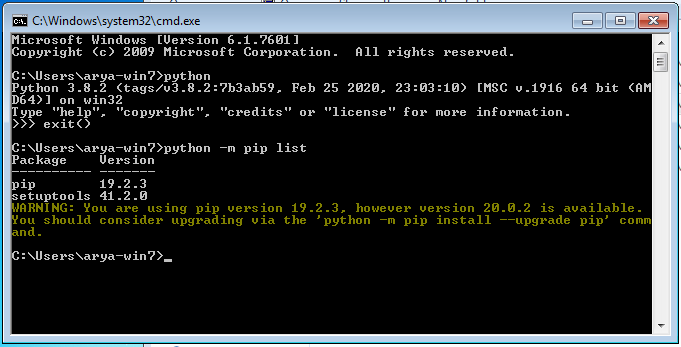
\includegraphics[scale=.5]{pics/pipList.png}
    \caption{Daftar paket yang terpasang}
    \label{fig:daftarPaket}
  \end{center}
\end{figure}

\texttt{pip} dapat juga digunakan untuk meng-\texttt{upgrade} paket yang telah terpasang, bahkan dirinya sendiri. Untuk meng-\textit{upgrade} paket \texttt{pip} itu sendiri, dapat dilakukan dengan menjalankan perintah \texttt{python -m pip install --upgrade pip} seperti \figurename~\ref{fig:pipUpgrade}. Perhatikan versi \texttt{pip} yang ada di \figurename~\ref{fig:daftarPaket} dan \figurename~\ref{fig:pipUpgrade}.
 
\begin{figure}
  \begin{center}
    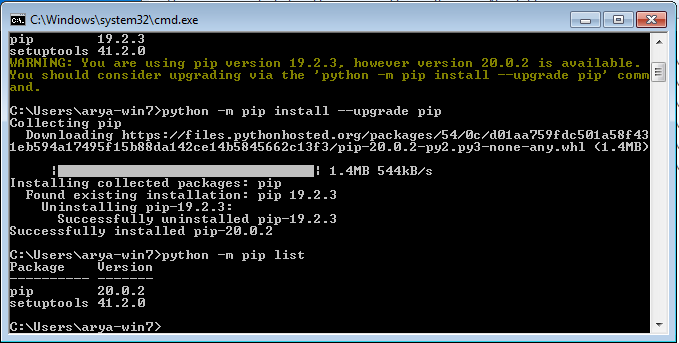
\includegraphics[scale=.5]{pics/pipList2.png}
    \caption{Hasil \texttt{upgrade} pip}
    \label{fig:pipUpgrade}
  \end{center}
\end{figure}

Sedangkan untuk memasang pustaka \texttt{scikit-image}, jalankan perintah \texttt{python -m pip install scikit-image} pada aplikasi \texttt{CMD} seperti \figurename~\ref{fig:installSkimage}.

\begin{figure}[h!]
  \begin{center}
    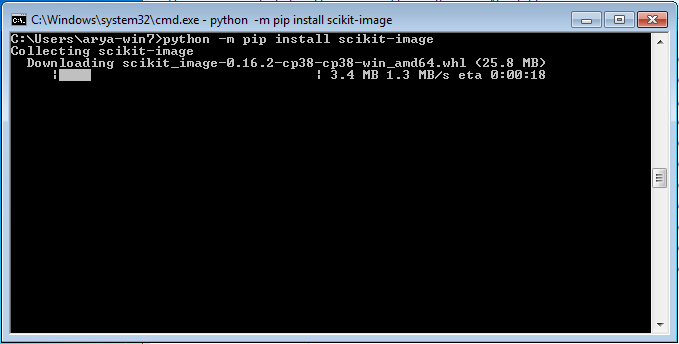
\includegraphics[scale=.5]{pics/installScikit-Image.png}
    \caption{Instalasi pustaka \texttt{scikit-image} menggunakan \texttt{pip}}
    \label{fig:installSkimage}
  \end{center}
\end{figure}

Jika ada pustaka lain yang menjadi ketergantungan dari pustaka yang akan diinstal, pip akan melakukan instalasi secara otomatis. \figurename~\ref{fig:installDepend} menunjukkan proses tersebut. Hal ini akan sangat memudahkan pengguna mengelola pustaka Python yang digunakan.

\begin{figure}[h!]
  \begin{center}
    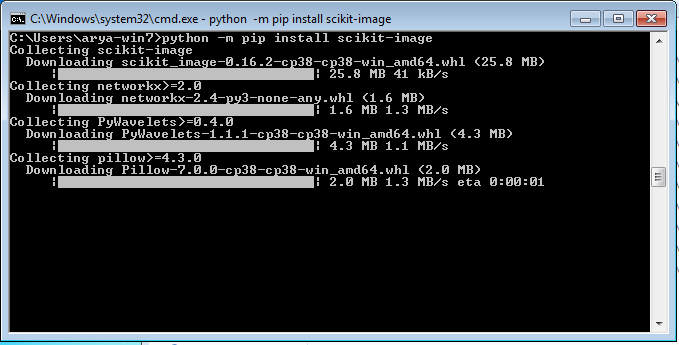
\includegraphics[scale=.5]{pics/installScikit-Imagedependencies.png}
    \caption{Instalasi pustaka \textit{dependent}}
    \label{fig:installDepend}
  \end{center}
\end{figure}

Setelah selesai, kita dapat kembali melihat daftar paket yang terpasang melalui pengelolaan \texttt{pip} yang ditunjukkan \figurename~\ref{fig:daftarPaket2}.

\begin{figure}[h!]
  \begin{center}
    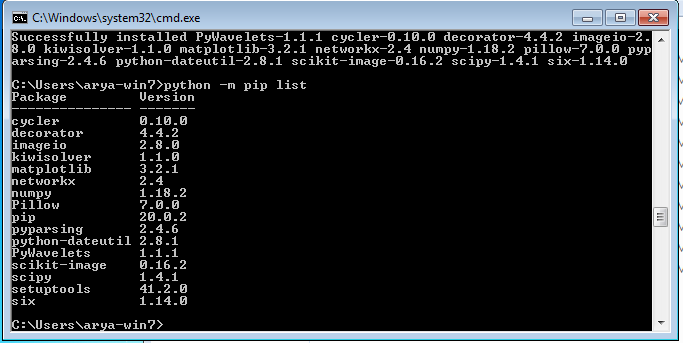
\includegraphics[scale=.5]{pics/pipList3.png}
    \caption{Daftar terakhir paket terpasang}
    \label{fig:daftarPaket2}
  \end{center}
\end{figure}

Menu aplikasi pendukung Python akan muncul seperti \figurename~\ref{fig:menu}. Menu kedua pada \figurename~\ref{fig:menu} akan memunculkan aplikasi \texttt{CMD} yang sama dengan yang ditunjukkan \figurename~\ref{fig:siap}, tetapi tanpa perlu memanggil perintah \texttt{python} terlebih dahulu. CMD secara otomatis akan memunculkan Python \texttt{shell} seperti \figurename~\ref{fig:siap}.

\begin{figure}[h!]
  \begin{center}
    \includegraphics[scale=.5]{pics/menuPython.png}
    \caption{Daftar menu aplikasi pendukung Python}
    \label{fig:menu}
  \end{center}
\end{figure}

\texttt{IDLE} adalah antarmukan \textit{interpreter} Python seperti ditunjukkan \figurename~\ref{fig:idle}. Dalam \figurename~\ref{fig:idle} juga terlihat bahwa kita berhasil meng-\textit{import} pustaka \texttt{scikit-image}, yang dalam \texttt{IDLE} di Windows 7 disebut sebagai \texttt{skimage}. Jika Anda sedang menggunakan Ubuntu, kemudian menggunakan pustaka \texttt{scikit-image} yang diperoleh dari \textit{repository} Ubuntu (bukan dari \texttt{pip}), pustaka \texttt{scikit-image} juga di-\textit{import} dengan nama \texttt{skimage}. Berhasilnya sebuah pustaka Python di-\textit{import} adalah ketika tidak ada komentar yang muncul setelah perintah \texttt{import} tersebut.

\begin{figure}
  \begin{center}
    \includegraphics[scale=.5]{pics/idle.png}
    \caption{Aplikasi \texttt{IDLE}}
    \label{fig:idle}
  \end{center}
\end{figure}

Selanjutnya, jika ditemukan petunjuk untuk masuk ke Python \texttt{Shell}, Anda dapat menggunakan aplikasi \texttt{IDLE}\texttt{}, atau menggunakan terminal (di Linux)/\texttt{CMD} (di Windows) dengan terlebih dahulu menjalankan perintah \texttt{python}.

\section{Anaconda}
Selain pilihan manual seperti yang telah dijelaskan di Sub bab \ref{sec:interpreter}, Anaconda bisa menjadi opsi lain yang lebih bersifat otomatis. Saya menyebutnya otomatis karena Anaconda sejumlah pustaka Python, terutama yang banyak digunakan di \textit{Data Mining}, \textit{Machine Learning} atau \textit{Data Science} telah dikemas di dalam Anaconda. Bahkan beberapa editor yang populer untuk Python juga dikemasnya. Anaconda bahkan mengemasnya khusus untuk \textit{platform} yang berbeda. Anda dapat menghubungi alamat \url{https://www.anaconda.com/} untuk mengunduh aplikasinya. Sesuaikan kebutuhan Anda dengan pilihan yang ada seperti ditunjukkan \figurename~\ref{fig:platformAnaconda}.

\begin{figure}[h!]
  \begin{center}
    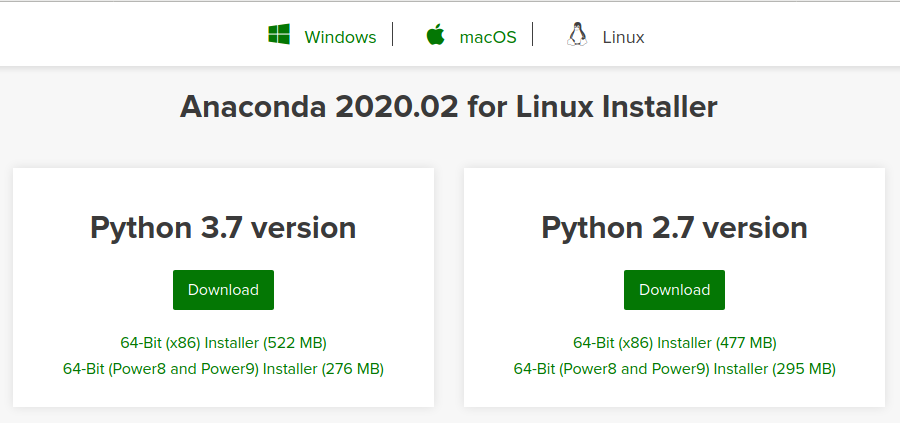
\includegraphics[scale=.5]{pics/anacondaInstall0.png}
    \caption{Pilihan \textit{platform} instalasi Anaconda}
    \label{fig:platformAnaconda}
  \end{center}
\end{figure}

Instalasi Anaconda akan menghadirkan dialog seperti ditunjukkan \figurename~\ref{fig:pembuka} - \figurename~\ref{fig:instalasiEnd}. Anaconda akan meletakkan pustaka di lokasi \texttt{C:\textbackslash\textbackslash ProgramData\textbackslash\textbackslash Anaconda3} yang berbeda dengan \texttt{pip} seperti terlihat di \figurename~\ref{fig:target}. Sedangkan di \figurename~\ref{fig:prosesInstalasi} terlihat sejumlah pustaka penting seperti \texttt{scikit-image} dan \texttt{scikit-learn} tengah diinstal. 

\begin{figure}aplikasi ini akan menghadirkan antarmuka seperti tampak
  \begin{center}
    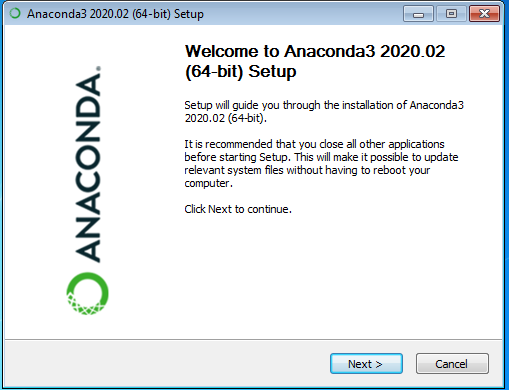
\includegraphics[scale=.5]{pics/anacondaInstall1.png}
    \caption{Dialog pembuka instalasi}
    \label{fig:pembuka}
  \end{center}
\end{figure}

\begin{figure}[h!]
  \begin{center}
    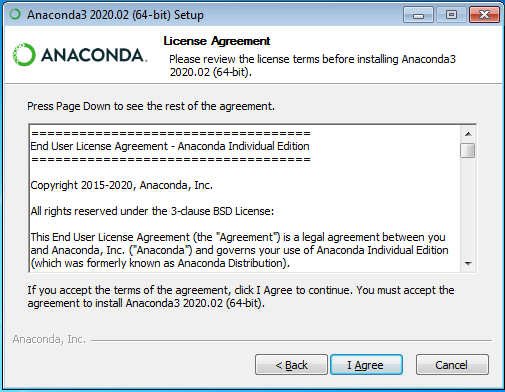
\includegraphics[scale=.5]{pics/anacondaInstall2.png}
    \caption{Menyetujui kesepakatan}
    \label{fig:kesepakatan}
  \end{center}
\end{figure}

\begin{figure}[h!]
  \begin{center}
    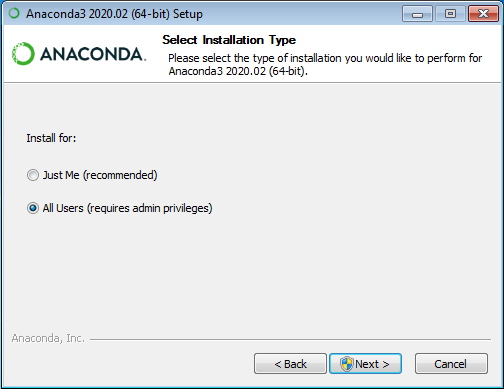
\includegraphics[scale=.5]{pics/anacondaInstall3.png}
    \caption{Pilihan pengguna Anaconda}
    \label{fig:pengguna}
  \end{center}
\end{figure}

\begin{figure}[h!]
  \begin{center}
    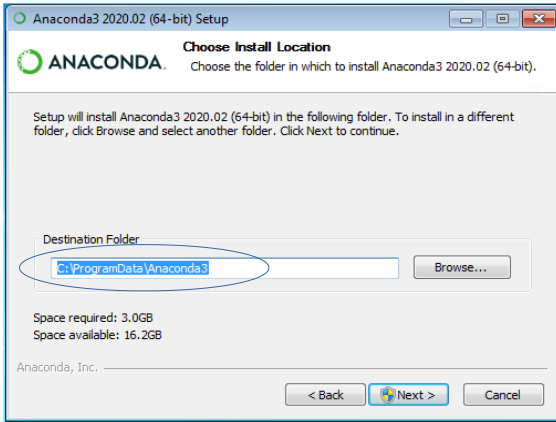
\includegraphics[scale=.5]{pics/anacondaInstall4a.png}
    \caption{Target instalasi}
    \label{fig:target}
  \end{center}
\end{figure}

\begin{figure}[h!]
  \begin{center}
    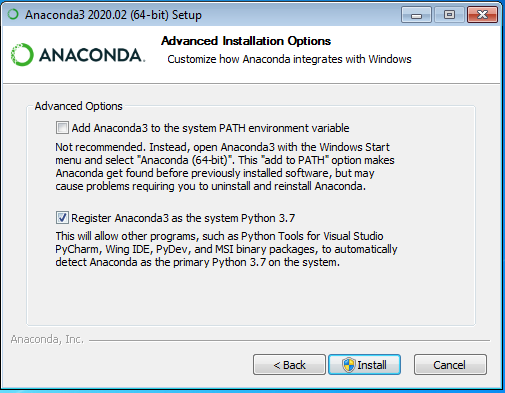
\includegraphics[scale=.5]{pics/anacondaInstall5.png}
    \caption{Menjadikan Anaconda sebagai sistem utama Python}
    \label{fig:utama}
  \end{center}
\end{figure}

\begin{figure}[h!]
  \begin{center}
    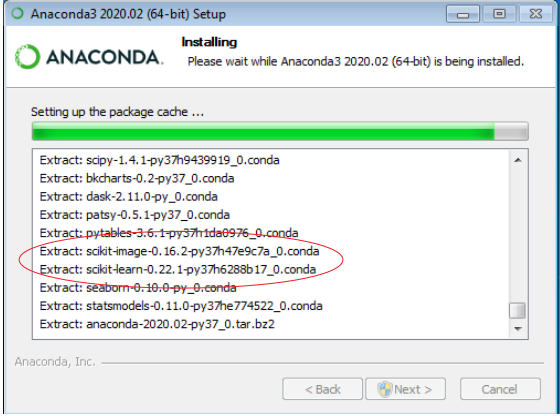
\includegraphics[scale=.5]{pics/anacondaInstall6a.png}
    \caption{Proses instalasi}
    \label{fig:prosesInstalasi}
  \end{center}
\end{figure}

\begin{figure}[h!]
  \begin{center}
    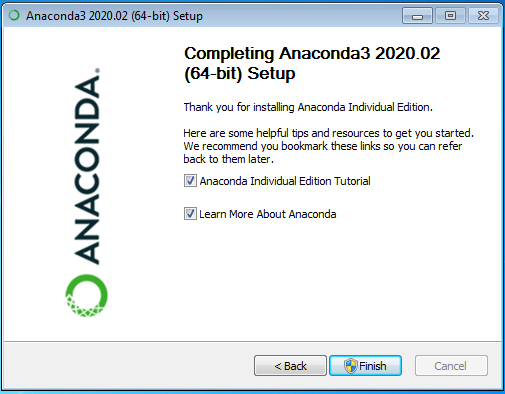
\includegraphics[scale=.5]{pics/anacondaInstall9.png}
    \caption{Instalasi selesai}
    \label{fig:instalasiEnd}
  \end{center}
\end{figure}

Instalasi Anaconda akan membuat menu seperti pada \figurename~\ref{fig:menuAnaconda}. Di situ terlihat sejumlah aplikasi yang dapat digunakan untuk mengembangkan kode komputer berbasis Python seperti Jupyter dan Spyder. Untuk Jupyter, aplikasi ini akan menghadirkan antarmuka seperti tampak pada \figurename~\ref{fig:jupyter}. Di sisi kanan atas terlihat beberapa opsi antarmuka untuk mengelola proyek Python dengan Jupyter, seperti Terminal \figurename~\ref{fig:jupyterTerminal} atau Python \texttt{Shell} di bawah Jupyter seperti \figurename~\ref{fig:jupyterShell} yang perannya seperti \texttt{IDLE} di \figurename~\ref{fig:idle}. Sedangkan untuk Spyder, akan tampak antarmuka seperti \figurename~\ref{fig:spyder}.

\begin{figure}[h!]
  \begin{center}
    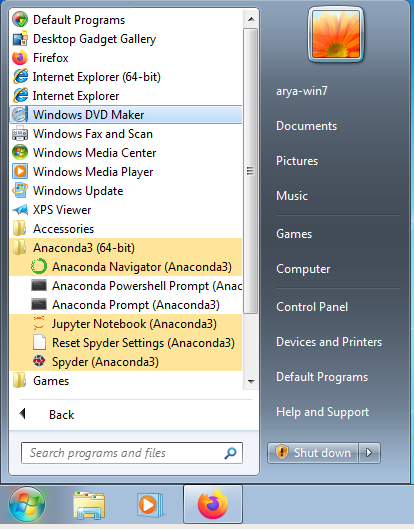
\includegraphics[scale=.5]{pics/anacondaMenu2.png}
    \caption{}
    \label{fig:menuAnaconda}
  \end{center}
\end{figure}

\begin{figure}
  \begin{center}
    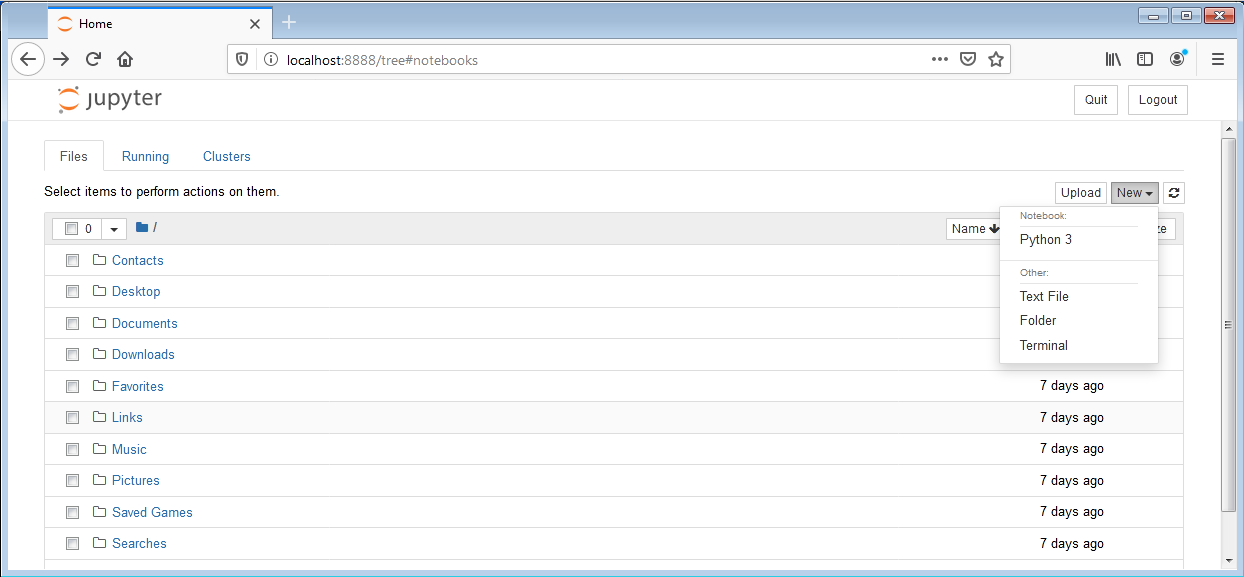
\includegraphics[scale=.5]{pics/jupyter2.png}
    \caption{Aplikasi \texttt{Jupyter}}
    \label{fig:jupyter}
  \end{center}
\end{figure}

\begin{figure}
  \begin{center}
    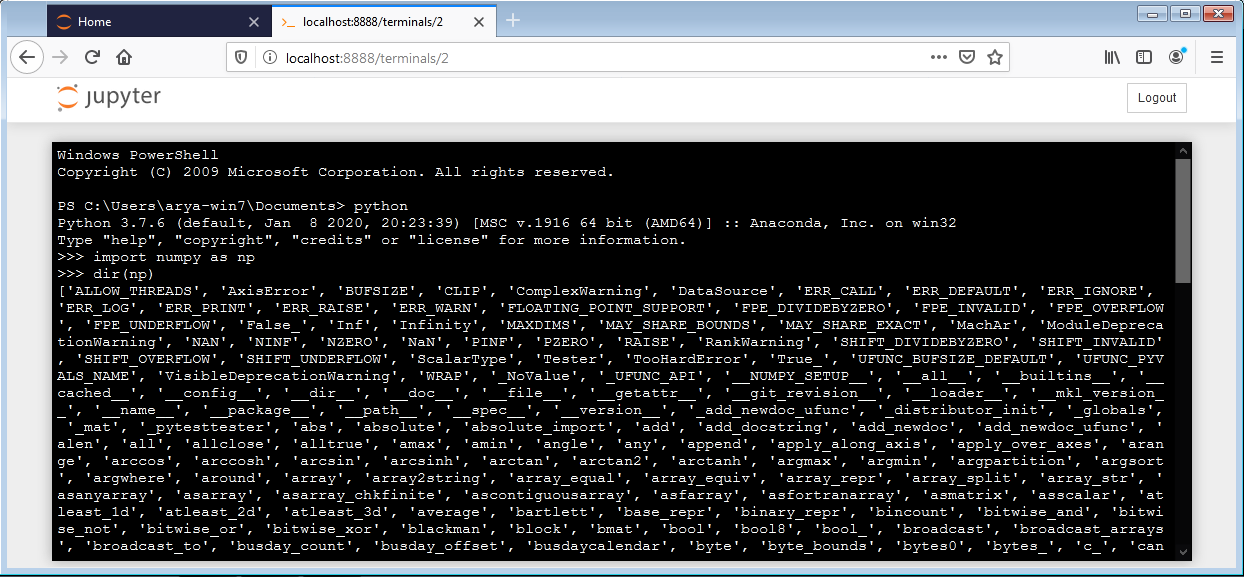
\includegraphics[scale=.5]{pics/jupyter3.png}
    \caption{Terminal pada aplikasi \texttt{Jupyter}}
    \label{fig:jupyterTerminal}
  \end{center}
\end{figure}

\begin{figure}
  \begin{center}
    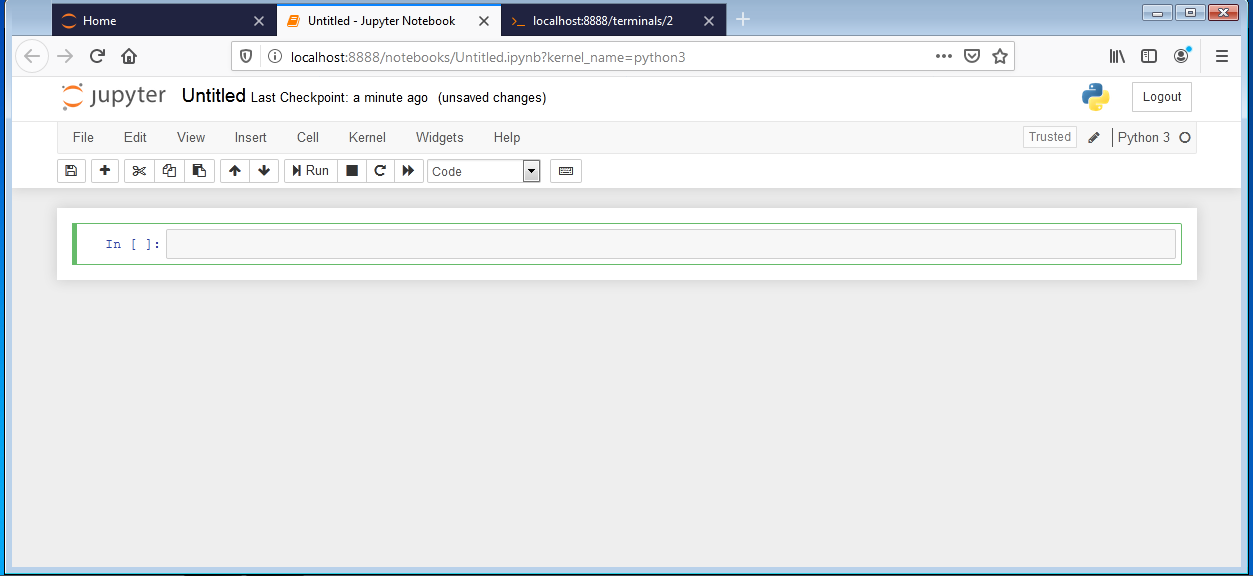
\includegraphics[scale=.5]{pics/jupyter4.png}
    \caption{Python \texttt{Shell} pada aplikasi \texttt{Jupyter}}
    \label{fig:jupyterShell}
  \end{center}
\end{figure}

\begin{figure}[h!]
  \begin{center}
    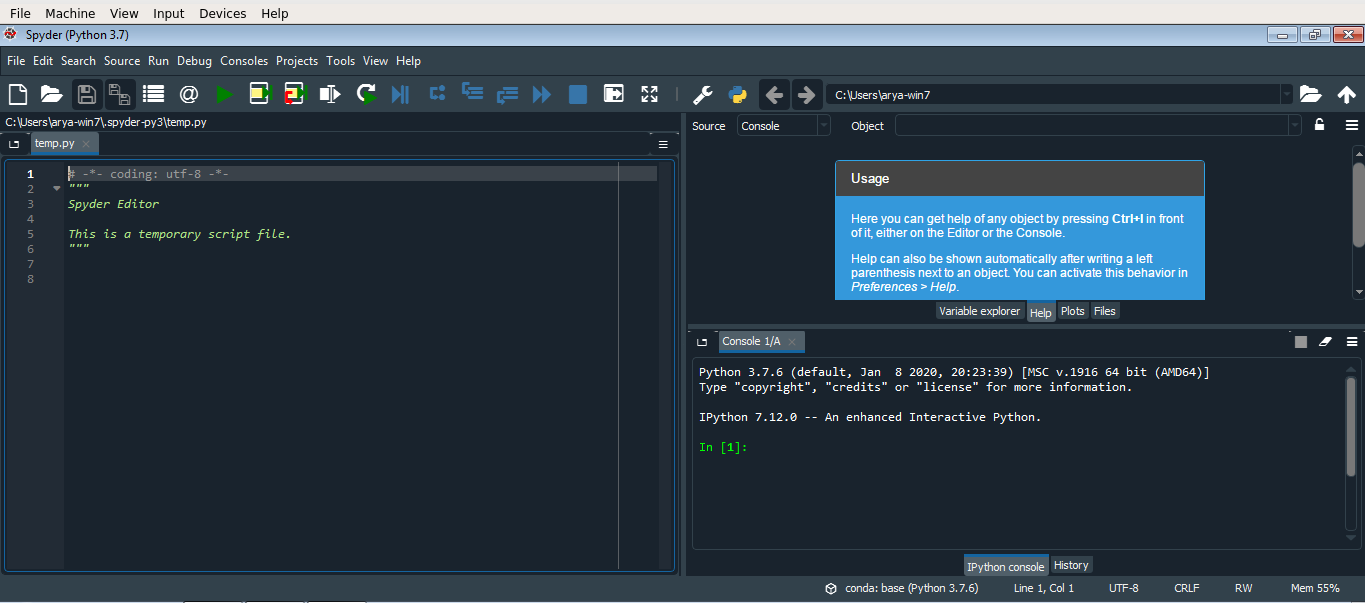
\includegraphics[scale=.45]{pics/spyder.png}
    \caption{Aplikasi \texttt{Spyder}}
    \label{fig:spyder}
  \end{center}
\end{figure}


\chapter{Dasar Pemrograman Python}

\chapter{Pendahuluan Pustaka \texttt{Scikit-Image}}

\chapter{Sub Modul Pustaka \texttt{Scikit-Image}}


\chapter{Pencarian (\textit{Searching})}

\bibliographystyle{apalike}
\bibliography{reference}
\end{document}
